\documentclass{beamer}
\usetheme{Madrid}
\AtBeginSection[]{
  \begin{frame}
  \vfill
  \centering
  \begin{beamercolorbox}[sep=8pt,center,shadow=true,rounded=true]{title}
    \usebeamerfont{title}\insertsectionhead\par%
  \end{beamercolorbox}
  \vfill
  \end{frame}
}

\AtBeginSubsection[]{
  \begin{frame}
  \vfill
  \centering
  \begin{beamercolorbox}[sep=8pt,center,shadow=true,rounded=true]{title}
    \usebeamerfont{title}\insertsubsectionhead\par%
  \end{beamercolorbox}
  \vfill
  \end{frame}
}



\usepackage{subcaption}
\usepackage{tikz}
\usetikzlibrary{positioning} 
\usetikzlibrary{matrix}
\usetikzlibrary{calc}
\newcommand{\z}{\mathbf{z}}
\newcommand{\uout}{u_{out}}
\newcommand{\vout}{v_{out}}
\newcommand{\uoutdum}{u_{out}^{dum}}
\newcommand{\uinplus}{u_{in}^{+}}
\newcommand{\uinminus}{u_{in}^{-}}
\newcommand{\winl}{w_{in}^{l}}
\newcommand{\win}{w_{in}}
\newcommand{\uin}{w_{in}}
\newcommand{\vin}{v_{in}}

\DeclareMathOperator*{\plusrightarrow}{\ensuremath{\xrightarrow{+}}}
\DeclareMathOperator*{\minusrightarrow}{\ensuremath{\xrightarrow{-}}}
\DeclareMathOperator*{\plusleftarrow}{\ensuremath{\xleftarrow{+}}}
\DeclareMathOperator*{\minusleftarrow}{\ensuremath{\xleftarrow{-}}}
\usetikzlibrary{shadows,positioning}
\colorlet{colD}{red!40}
\colorlet{colIP}{cyan!40}
\colorlet{colV}{blue!40}
\colorlet{colBorder}{gray!70}


\title[SLIDE]{MLDB Presentation\\SLIDE: Sub-LInear Deep Learning Engine}

\author[Beidi Chen et al.]{Beidi Chen \and Tharun Medini \and James Farwell \and Sameh Gobriel \and Charlie Tai \and Anshumali Shrivastava}
\date{\today}

\begin{document}
\begin{frame}
    \titlepage
\end{frame}

\begin{frame}
    \frametitle{Overview}
    \tableofcontents
\end{frame}


\section{Motivation}
\begin{frame}
    \frametitle{Era of Deep Learning}
    \begin{figure}[ht!]
        \centering
        \begin{subfigure}{0.4\textwidth}
            \centering
            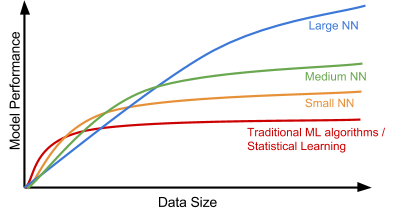
\includegraphics[width=1.2\textwidth]{images/deep learning.png}
            \caption{Model Performance wrt Dataset size}
            \label{fig:deep-learning}
        \end{subfigure}
        \begin{subfigure}{0.4\textwidth}
            \centering
            
\includegraphics[width=0.7\textwidth]{images/xkcd.png}
            \caption{Fun xkcd comic}
            \label{fig:deep-learning}
        \end{subfigure}

    \end{figure}
    
\end{frame}
\begin{frame}
    \frametitle{Trends}
    \begin{itemize}
        \item Large datasets $\rightarrow$ More Data
        \item Big models (Eg, 17B parameter NLP models)
        \item Improvements in optimizations and gradient descent
        \item \structure{Matrix multiplication} is a computational bottleneck
        \item Many approaches exists such as \structure{GPUs}
    \end{itemize}

\end{frame}

\subsection{Existing Approaches}
\begin{frame}
    \frametitle{Low Rank structure}

    \begin{minipage}{0.6\textwidth}
        \begin{itemize}
            \item $W \in \mathbb{R}^{m\times n}$ is weight matrix
            \item $W$ has a low-rank structure $W=UV$
            \item $U\in \mathbb{R}^{m\times r}$ and $V\in \mathbb{R}^{r\times n}$, where $r \ll \min(m,n)$
            \item Equivalent representation with $I$ activation function is better
            \item $\mathcal{O}(mn)$ becomes $\mathcal{O}(mr+rn)$
            \item \structure{Better storage} of parameters as well
            \item But still needs dense gradient update, cannot parallelise asynchronously
        \end{itemize}
    \end{minipage}\hfill
    \begin{minipage}{0.4\textwidth}
        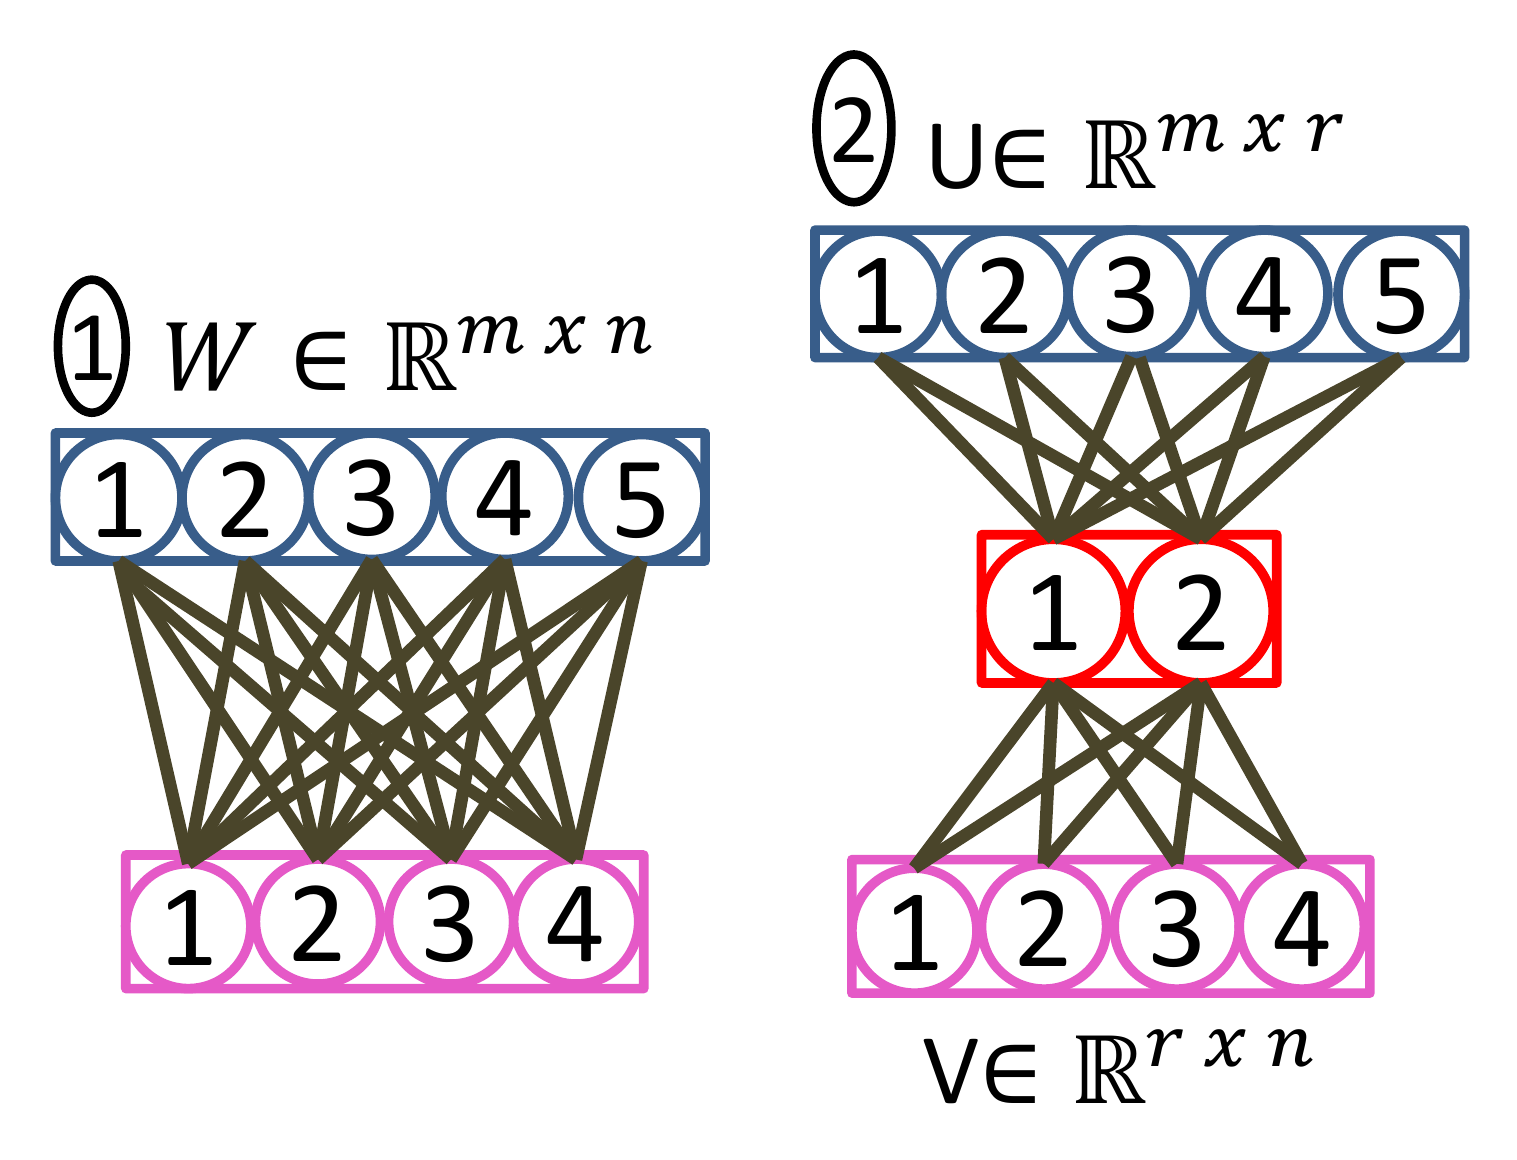
\includegraphics[width=\textwidth]{images/Low_Rank.png}
    \end{minipage}

\end{frame}

\begin{frame}
    \frametitle{Dropout and Sparsity}
    \begin{minipage}{0.5\textwidth}
        \begin{itemize}
            \item Well known regularization method for Neural Networks
            \item With probability $p$ neurons in each layer is \structure{turned off}
            \item Used during training to ensure model generalizes 
            \item Sparsity above 50\% tends to begin hurting performance
        \end{itemize}
    \end{minipage}\hfill
    \begin{minipage}{0.5\textwidth}
        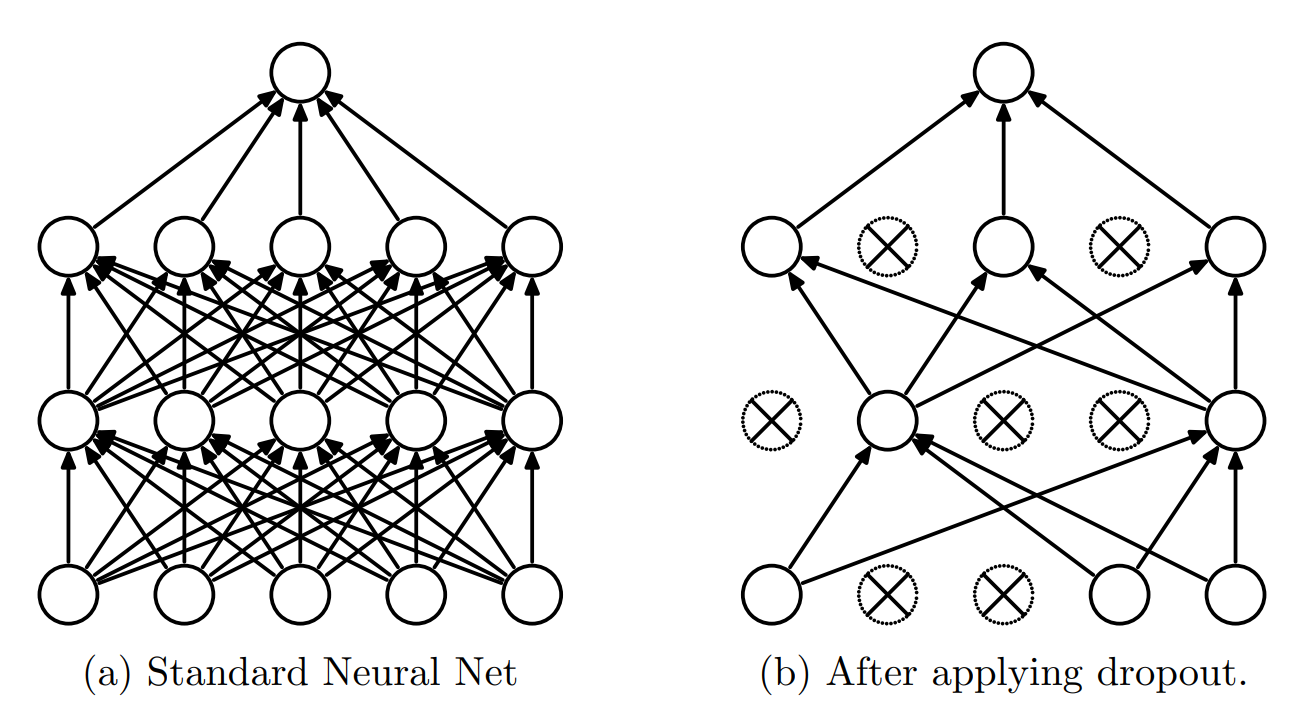
\includegraphics[width=\textwidth]{images/dropout.png}
    \end{minipage}
    
\end{frame}

\begin{frame}
    \frametitle{Adaptive Dropout}
    \begin{itemize}
        \item \cite{Lei_adaptive_dropout}
    \end{itemize}
    

\end{frame}
\subsection{Problem Setting}

\section{Contributions}
\begin{frame}
    \frametitle{Main Contributions}

    \begin{itemize}
        \item C++ OpenMP implementation for "standard" CPU
        \item Sparsity inspired, LSH based backpropagation algorithm
        \item Rigorous evaluation with TF-GPU and CPU
        \item Further optimizations using Hugepages and SIMD instructions
    \end{itemize}
    

\end{frame}

\section{Locality Sensitive Hashing}
\subsection{Sampling Approach to LSH}
\subsection{Additional Optimizations}

\section{Implementation}



\section{Results}

\begin{frame}
    \frametitle{}

    \centering \Large
    \emph{Questions or Comments}

\end{frame}

\bibliography{sources}
\bibliographystyle{apalike}
\end{document}